\section{Introduction}
\label{sec:introduction-cell}

In the model outlined in Chapter \ref{cha:stamm} and applied to two biological systems in Chapters \ref{cha:oncog-transf} and \ref{cha:stem-cells} the initial cell population is assumed to be homogeneous. In the two applications discussed before this assumption is warranted due to experimental design. In the case of the oncogenic transformation the experiment is started from a cell line ensuring homogeneity. In the case of stem cell reprogramming the technique outlined by \cite{Hanna:2009ix} tries to ensure initial homogeneity  by using a secondary MEF cells.

Recently it has been shown that even seemingly homogeneous cell populations have an inherent mixture, be it at an epigenetic level \citep{Heng:2009em,Gerlinger:2012wu}. In this Chapter we outline a model that answers the question: What effect does the initial cell population have on cell fate?


\begin{figure}[h]
  \centering
  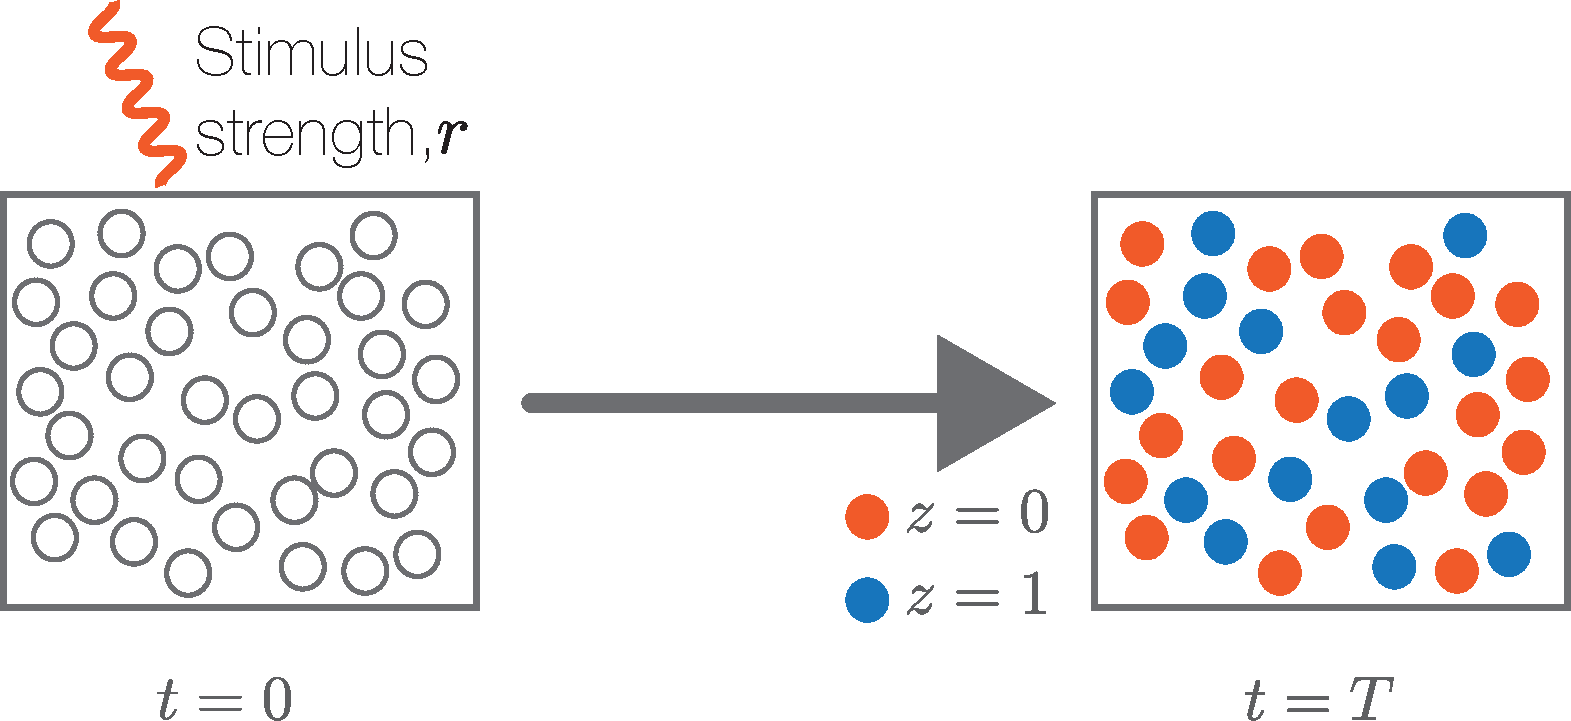
\includegraphics[width=0.7\textwidth]{pics/cell-cycle-model.pdf}
  \caption{Schematic of heterogeneous cell population transforming under stimulus.}
  \label{fig:cell-cycle-model}
\end{figure}

An example of such a biological system is one with an initial heterogeneous cell population made up of two types of cells, with an indistinguishable phenotype. At time $t=0$ the cells receive a stimulus leading to a transformation such that at $t=T$ it is possible to distinguish cells in their final cell fate. Now it is possible to count the fraction of cells that reach each of those final cell fates. The interesting case here is when the strength of the stimulus has an affect on the fraction of cells in each cell fate. A schematic of such a system is shown in Figure \ref{fig:cell-cycle-model}. Individual genes are influential in determining cell fate if their expression level is significantly different between cell populations at $t=0$. 

% The question we try to answer in this chapter is, "what if the initial population is heterogeneous?". 

\section{Formal system description}
\label{sec:model-descr}

\subsection{Concepts}
\label{sec:concepts}

% To formalise model description we derive it

Suppose at time $t$ cell $i$ (out of $N$ cells) occupies state $X_{it}$; where state here broadly refers to any aspect of the cell's physical configuration. This can include protein profile, transcription, or its chromatin state. Denote ultimate cell fate at $t=T$ for cell $i$ by $Z_i$. Cell fate $Z_i$ is determined experimentally by enumerating cells in distinguishable states at $t=T$. In the simplest case cells can have two distinct final states; we label the two states $Z_i = 0$ and $Z_i = 1$. We expect the process that determines cell fate to have a stochastic component such that two physically identical cell at $t=0$ can end up in distinct final states. Hence we assume the probability that cell $i$ is in state $Z_i = 1$ at $t=T$ depends on two things:

\begin{itemize}
\item The physical state of cell $i$ at $t=0$, $X_{i0}$.
\item The dose of the stimulus $r$. 
\end{itemize}

Since we assume that the fraction of cells that reach the arrested state changes with the strength of the stimulus. The fraction of cells that reach cell fate $Z_i = 1$ is dose dependant and denoted by $\pi(t)$.

\subsection{Model}
\label{sec:model-cell}



%%% Local Variables:
%%% TeX-master: "warwickthesis"
%%% End: